% LaTeX Datei f�r Projektarbeiten etc. am MZH

% ------------------------------------------------------------------------------------------
% erlaubt das Anfangen des Draft-Modus und damit Ver�nderungen
% einzustellen
\newif\ifdraft
% Draft-Modus: Arbeitsversion, Bilder werden nur als Rahmen dargestellt
% Vorteil: schnelleres Kompilieren
%\drafttrue % <- daf�r hier die Kommentierung wegnehmen

%-------------------------------------------------------------------------------------------
% folgende Befehle sorgen daf�r, das f�r jede Schrift die richtigen Pakete installiert werden
\newcounter{schrift}
% Schrift ausw�hlen:
% 1 - mathptmx
% 2 - minionpro
% 3 - mathpazo
% 4 - times + computer modern
% 5 - computer modern
\setcounter{schrift}{4} % Hier die entsprechende Zahl setzen !

% ------------------------------------------------------------------------------------------
% ------------------------------------------------------------------------------------------
% Latex - Pr�ambel
% hier werden alle wichtigen Dokumenteinstellungen getroffen, normalerweise m�ssen
% keine �nderungen mehr durchgef�hrt werden.
% Pakete die das Schriftbild, den Satzspiegel oder die R�nder ver�ndern, d�rfen
% nicht hinzugef�gt werden, erst nach Abstimmung mit dem Betreuer.
% n�tzliche Pakete sind willkommen, bitte die Wiki entsprechend aktualisieren
% viele Pakete sind drin, die vielleicht nicht jeder braucht und das Kompilieren verl�ngern
% sollten diese das Layout nicht ver�ndern, k�nnen diese nat�rlich auskommentiert werden.
% ------------------------------------------------------------------------------------------

% ------------------------------------------------------------------------------------------
% Dokumentenklasse definieren:
\ifdraft
    \documentclass[draft, 
                   paper=a4,
                   BCOR5mm,
                   fontsize=12pt, 
                   DIV13, 
                   headsepline, 
                   numbers=noenddot, 
                   %bibtotoc,
                   bibliography = totoc,
                   %version=first,
                   %smallheadings,
                   headings = small,
                   oneside]{scrbook}
\else
    \documentclass[paper=
                   a4,
                   BCOR5mm,
                   fontsize=12pt, 
                   DIV13, 
                   headsepline, 
                   numbers=noenddot, 
                   %bibtotoc,
                   bibliography = totoc, 
                   %version=first,
                   %smallheadings,
                   headings = small,
                   headinclude=true,
                   footinclude=false,
                   fleqn, % formeln links b�ndig
                   oneside]{scrbook}
\fi
% Standard-Koma-Dokument mit
%   Papierformat A4
%   Binderand 5 mm
%   Schrift 12-Punkt
%   Seitenlayout nach DIV, siehe scrguide.pdf text b/h rand oben/innen: 168,00 237,60 19,80 14,00 (ist raus)
%   Linie unter der Kopfzeile
%   Nummern ohne Punkt am Ende
%   Literaturverzeichnis im Inhaltsverzeichnis
%   �berschriften etwas kleiner als standard
%   weitere Informationen zum Koma-Skript: www.komascript.de

%---------------------------------------------------------------
% Basis-Pakete
%---------------------------------------------------------------
\usepackage{ifpdf}		%   Ueberprueft, ob LaTeX oder pdfLaTeX verwendet wird (nur ab MikTeX 2.5)
\usepackage[T1]{fontenc}        %   8-Bit-Fonts
\usepackage{textcomp,latexsym}  %   zusaetzliche Symbole
\usepackage[ansinew]{inputenc}   %   Quelltext ist Latin-1 (d.h. Windows-) kodiert
\usepackage[ngerman]{babel}            %   neue deutsche Rechtschreibung
\usepackage{scrtime}            %   fuer die aktuelle Zeit
%\usepackage{scrdate}            %   fuer das aktuelle Datum
%\usepackage{natbib}             %   Literaturverweise mit (Autor Jahr) nach DIN
%\bibpunct[; ]{[}{]}{,}{a}{}{;}  %   eckige Klammern statt runde bei Zitaten
%\usepackage[T1]{url}            %   Web-Addressen auch mit T1-Encoding
%\urlstyle{tt}                   %   und in tt-Font
%\usepackage[activate=normal]{pdfcprot} % dient dem optischen Randausgleich bei k�rzeren Zeichen wie '-', '.', ',', '!'

\usepackage{color}

\PassOptionsToPackage{x11names}{xcolor}
\usepackage{xcolor}


%---------------------------------------------------------------
% n�tzliche Zusatz-Pakete
%---------------------------------------------------------------
%\usepackage{makeidx}            %   Index (wenn gewuenscht)

\usepackage{setspace}           %   Zeilenabstand setzen. Befehl:
                                %   \begin{spacing{Wert}
                                %   Text
                                %   \end{spacing}
%\usepackage{placeins}           %   das Positionieren von float-Umgebungen bestimmen:
                                %   der Befehl \floatbarrier sorgt daf�r, dass alle vorher eingegebenen
                                %   float-Umgebungen VOR diesem Befehl eingef�gt werden.
                                
%\usepackage{subfig}          %   Bilder gruppieren, mehrere Bilder in einer Umgebung einf�gen
                                %   Bsp.:
                                %   \begin{figure}
                                %   \centering
                                %    \subfloat[Text a]
                                %    {\includegraphics{bild a}}
                                %    \subfloat[text b]
                                %    {\includegraphics{bild b}}
                                %    \caption{Untertitel}
                                %    \label{fig.Beziechnung_subfigure} <- am besten mit fig. dann kann mit \bild{Bezeichnung_figure} referenziert werden
                                %   \end{figure}                                

%\usepackage{textcomp}           %   fuer Trademark und Copyright Zeichen
                                %   z.B \texttrademark, \textregistered, \texteuro etc.

\usepackage{tabularx}           %   erweiterte Funktionen f�r Tabellen

\usepackage{longtable}          %   Longtable-Package f�r Tabellen die l�nger als eine DIN-A4-Seite sind

\usepackage{colortbl}						%		farbige Tabellenzeilen

\usepackage{nicefrac}           %   Schr�ge Bruchstriche \nicefrac{Nenner}{Z�hler}

%\usepackage{numprint}           %   Zahlen mit Einheiten n�her an der Zahl/kein Umbruch und 1 000er Format \numprint[Einheit]{Zahl}

%\usepackage{mathcomp}           %   f�r \tcdegree (� Gradzeichen bei numprint) \numprint[\tcdegree]{180} f�r 180�

%\usepackage{hhline}             %   hhline-Package
                                %   Fuer komplexe Linienzuege in Tabellen \hhline{}
                                %   = Spalte mit doppelter Linie      | vertikale Linie die horizontale schneidet
                                %   - Spalte mit einfacher Linie      : vertikale Linie die von horizantaler unterbrochen ist
                                %   ~ Spalte ohne Linie               # doppelte horiz. geschnitten mit doppelter vert. Linie
                                %   t oberer Teil ->                  b unterer Teil einer doppelten Linie

%\usepackage[active]{srcltx}     %   bei verwendung v. \includeonly spring winedt jetzt bei fehlern an die richtige stelle

\usepackage{flafter}            %   Ein float-Objekt immer erst NACH seiner Definition platzieren

\usepackage{ifthen}             %   definiert \ifthenelse{}{}{}

%\usepackage{path}               %   dateinamen und pfade darstellen

%\usepackage{pdfsync}						%   Synchronisation mit SumatraPDF <<-- geht auch ohne

\usepackage{booktabs}

%% Eigene Pakete

\usepackage{scrhack} % L�scht Warnungen von Packages wie hyperref, listings
\usepackage[ locale = DE,            % deutsch
            load-configurations=abbreviations, % zus�tzliche Einheiten siehe manual
            per-mode=symbol,%-or-fraction,
            separate-uncertainty% 
            ]
            {siunitx}								% SI-Einheiten  

            
\usepackage{multirow}               % zwei Zeilen kombinieren (wie multicolumn)
\usepackage[babel]{microtype}       % schickeres Schriftbild -> aber l�ngeres Kompilieren

\usepackage{blindtext}							% sinnlosen text einbauen
\usepackage{subfigure}

\usepackage{newunicodechar}
%\newunicodechar{ }{~}

%\DeclareUnicodeCharacter{00A0}{~}


%%

%---------------------------------------------------------------
% Grafik-Paket f�r eps bzw. pdf
%---------------------------------------------------------------
% �berpr�ft ob Latex oder PDFLatex ausgef�hrt wird, dementsprechend werden pdf/jpg oder eps Bilder eingef�gt
% sollen dvi oder pdf Dokumente erstellt werden m�ssen alle Bilder in beiden Formaten vorliegen
% hierf�r gibt es Tools wie epstopdf oder jpgtoeps
 \ifdraft
    \usepackage[draft]{graphicx}
\else
    \ifpdf
        \usepackage{graphicx}
        \usepackage{pgfplots} % pgfplots zum plotten in LaTeX
    \else
        \usepackage[final]{graphicx}
    \fi
\fi
% von wo sollen die Grafiken kommen?
\graphicspath{{./fotos/}{./skizzen/}{./zeichnungen/}{./plots/}}

%Einstellungen f�r pgfplots
\pgfplotsset{compat=1.3,
	%enlargelimits=auto,
	tick label style={font=\small,/pgf/number format/use comma}, %Komma nutzen in allen Axen
	%axis x line=center, %alle x-Achsen center
	%axis y line=center, %alle y-achsen center
	%every axis x label/.style={at={(current axis.right of origin)},anchor=west}, % achsenbeschriftung bei allen x-achsen rechts
	%every axis y label/.style={at={(current axis.above origin)},anchor=south},   % achsenbeschriftung bei allen y-achsen oben
	%every x tick scale label/.style={at={(current axis.right of origin)},anchor=north,yshift=-0.5em}, %positionierung des scale faktors ge�ndert
	every axis legend/.append style={at={(0.5,1.03)},anchor=south,nodes=right,font=\small}, % Legende �ber der Grafik, schriftgr��e small
	label style={font=\small} % label schriftgr��e small
}
\newlength\tikzwidth
\setlength{\tikzwidth}{0.7\textwidth}
\definecolor{mycolor1}{rgb}{0,0.5,0}

\ifpdf
 \ifdraft
    \usepackage[draft]{pdfpages}%   externe PDF Seiten einbinden nur bei PDF-Latex m�glich
    \else
    \usepackage[final]{pdfpages}%   externe PDF Seiten einbinden nur bei PDF-Latex m�glich
 \fi                            %   Befehl: \includepdf{PDF-Datei} soll die Datei im Querformat angezeigt werden
    \else
\fi                             %   \includepdf[landscape=true]{PDF-Datei}

%---------------------------------------------------------------
% Debug-Ausgabe der Labels und References
%---------------------------------------------------------------
\ifdraft
  \usepackage{showkeys} % Label werden im Draft Modus im Text angezeigt
\fi

%---------------------------------------------------------------
% Abweichende PostScript-Schriftarten
% werden in der main Datei ausgew�hlt, hier nichts �ndern
%---------------------------------------------------------------
\ifthenelse{\equal{ 1 }{ \value{schrift} }}
    {
    \usepackage{mathptmx}          %   Times als Hauptschriftart, keine mathematische Fettschrift
    \usepackage{amssymb}
    \usepackage{amsbsy}
    \usepackage{amsmath}
    \usepackage{amsfonts}
    \usepackage{amstext}
    \renewcommand{\boldsymbol}[1]{\mathbf{#1}} % nur bei mathptmx !
                                               % damit boldsymbol wenigstens fette aufrechte Buchstaben macht
    }{}
\ifthenelse{\equal{ 2 }{ \value{schrift} }}
    {
    \usepackage[lf, minionint]{MinionPro} %   OpenType von Adobe, mathematische Fettschrift vorhanden, Schrift ist
                                %   ist im Standard-LaTeX nicht installiert.
                                %   Ist ein wenig Aufwand das Ganze zu installieren, Matthias Dagen fragen
    }{}
\ifthenelse{\equal{ 3 }{ \value{schrift} }}
    {
    \usepackage{mathpazo}          %   nette Buchschrift aber sehr gross, mathematische Fettschrift vorhanden
    \usepackage{amssymb}
    \usepackage{amsbsy}
    \usepackage{amsmath}
    \usepackage{amsfonts}
    \usepackage{amstext}
    }{}
\ifthenelse{\equal{ 4 }{ \value{schrift} }}
    {
    \usepackage{times}
    \usepackage{amssymb}
    \usepackage{amsbsy}
    \usepackage{amsmath}
    \usepackage{amsfonts}
    \usepackage{amstext}
    }{}
\ifthenelse{\equal{ 5 }{ \value{schrift} }}
    {
    \usepackage{amssymb}
    \usepackage{amsbsy}
    \usepackage{amsmath}
    \usepackage{amsfonts}
    \usepackage{amstext}
    \usepackage{lmodern}
    }{}
\usepackage[scaled=.92]{helvet} %   11pt Helvetica f�r �berschriften etc. etwas kleiner da, Helvetica an sich gr��er ist
%\usepackage{courier}            %   Courier bei \texttt
%\usepackage{upgreek}            %   Aufrechte griechische Buchstaben

% ------------------------------------------------------------------------------------------
% Bild- und Tabellentitel FETT
% ------------------------------------------------------------------------------------------
%\def\figurename{\bfseries Bild}
%\def\tablename{\bfseries Tabelle}

%%Andere Beschreibung von figure
\addto\captionsngerman{
	\renewcommand{\figurename}{\bfseries Bild}%%Andere Beschreibung von figure
	\renewcommand{\listfigurename}{Bildverzeichnis}
	\renewcommand{\tablename}{\bfseries Tabelle}
}

%---------------------------------------------------------------
% Quelltexte formatieren
%---------------------------------------------------------------
\usepackage{listings}


%\lstloadlanguages{
		%C,
		%C++,
		%XML
%}

\lstset{
		language=XML,
		basicstyle=\footnotesize\ttfamily, % Standardschrift
		numbers=left,               % Ort der Zeilennummern
		numberstyle=\tiny,          % Stil der Zeilennummern
		numbersep=5pt,              % Abstand der Nummern zum Text
		tabsize=2,                  % Groesse von Tabs
		extendedchars=true,         %
		breaklines=true,            % Zeilen werden Umgebrochen        
		keywordstyle=\color{Red2},
		frame= b,         
		stringstyle=\color{Purple2}\ttfamily, % Farbe der String
		showspaces=false,           % Leerzeichen anzeigen ?
		showtabs=false,             % Tabs anzeigen ?
		xleftmargin=17.5pt,
		framexleftmargin=17pt,
		framexrightmargin=5pt,
		framexbottommargin=4pt,
		linewidth= \dimexpr\textwidth-2\fboxsep-2\fboxrule,
		comment=[l]{\#},
		morecomment=[s]{<!--}{-->},
		commentstyle=\color{Green4},
		%backgroundcolor=\color{grey},
		showstringspaces=false,      % Leerzeichen in Strings anzeigen ?        
		morekeywords={__global__, name, pkg, args, type, from, to, textfile, respawn, value, output, radius, ixx, ixy, ixz, iyy, iyz, xyz, rpy, reference},  % CUDA specific keywords
		aboveskip = 18pt, 
		belowskip = 18pt
}

\usepackage{caption}
\DeclareCaptionFont{white}{\color{white}}
\DeclareCaptionFormat{listing}{\colorbox{darkgray}{\parbox{\dimexpr\textwidth-2\fboxsep-2\fboxrule}{\hspace{15pt}#1#2#3}}}
\captionsetup[lstlisting]{format=listing,labelfont=white,textfont=white, singlelinecheck=false, margin=0pt, font={bf,footnotesize}}

%---------------------------------------------------------------
% ein paar L�ngen einstellen
%---------------------------------------------------------------
%\setlength{\parskip}{1ex plus0.5ex minus0.2ex} % Absatzabstand etwas gr��er
\setlength{\itemsep}{0ex plus0.2ex}            % Abstand zweier Listenelemente kleiner
\setlength{\parindent}{0ex}                     % kein Absatzeinzug
\setlength{\belowcaptionskip}{0.4cm}            % Abstand caption - Tabelle gr��er
\setlength{\abovecaptionskip}{0.4cm}            % Abstand caption - Tabelle gr��er

%---------------------------------------------------------------
% Kopf- und Fusszeilen
%---------------------------------------------------------------
\usepackage[plainheadsepline,  % linie zw. kopf und text auch bei seitenstil "plain"
           %headexclude,       % kopfzeile geh�rt nicht zum textk�rper
           %footexclude        % fusszeile geh�rt nicht zum textk�rper
          ]       
           {scrpage2}
\pagestyle{scrheadings}
\clearscrheadfoot              % voreinstellungen loeschen
\ihead{\normalfont\headmark}   % kolumnentitel innen
\ohead[\pagemark]{\pagemark}   % seitenzahl aussen

%---------------------------------------------------------------
% Nummerierungs-Tiefe des Inhaltsverzeichnis und der Abschnitte einstellen
%---------------------------------------------------------------
\setcounter{secnumdepth}{2} \setcounter{tocdepth}{2}

%---------------------------------------------------------------
% Abk�rzungsverzeichnis
%---------------------------------------------------------------
% mit dem Befehl \nomenclature[l/g/a]{Abk�rzung}{Bezeichnung} kann direkt im Code die Abk�rzung eingef�gt werden
% das Paket sortiert diese und f�gt sie mit dem Befehl \printnomenclature ein
% l, g, oder a steht dabei f�r die Gruppierung Lateinische bzw. Griechische Buchstaben, Abk�rzungen
% Nach Einf�gen neuer Abk�rzungen muss folgender Befehl in der Eingabeaufforderung im Tex-Verzeichnis eingegeben werden:
% -> vorher einmal kompilieren
% -> makeindex main.nlo -s nomencl.ist -o main.nls
% -> nochmal kompilieren
%\makeindex
\usepackage{nomencl}
% \let\abbrev\nomenclature
\renewcommand{\nomname}{Abk�rzungsverzeichnis}
\setlength{\nomlabelwidth}{.25\hsize}
\renewcommand{\nomlabel}[1]{#1 \hfill}
\setlength{\nomitemsep}{-\parsep}

\renewcommand{\nomgroup}[1]{%
	\ifthenelse{\equal{#1}{L}}{\item[\textbf{Lateinische Buchstaben}]}
	{%
		\ifthenelse{\equal{#1}{G}}{\item[\textbf{Griechische Buchstaben}]}
		{%
			\ifthenelse{\equal{#1}{A}}{\item[\textbf{Abk�rzungen}]}
			{
				\ifthenelse{\equal{#1}{K}}{\item[\textbf{Koordinatensysteme}]}{}
			}
		}
	}
}

\makenomenclature

%---------------------------------------------------------------
% Hyperlinks f�r pdfTeX
%---------------------------------------------------------------
\ifpdf
    % hier stehen befehle, die nur f�r pdftex gelten
    \usepackage[pdfpagelabels,  % logische (z.b. auch roemische) seitenzahlen
                bookmarks,       % Bookmarks f�r die einzelnen Abschnitte
                pdftex
                ]{hyperref}
    \hypersetup{
    %   colorlinks,  % Links mit farbigem Text
        pdfborder   = 0 0 0,
        plainpages  = false,
        bookmarksnumbered = true,
    %   bookmarksopen
    }
\else
    % hier stehen befehle, die nur f�r latex gelten
    \usepackage{hyperref} % hier ohne colorlinks und pdf-krams
\fi

%extra inhaltsverzeichnisse m�glich
\usepackage[nohints]{minitoc}     
\renewcommand{\mtctitle}{Anhangsverzeichnis} 				% Name �ndern            
\renewcommand{\mtifont}{\large\bfseries\sffamily}		% Titel font �ndern
\renewcommand{\mtcSfont}{\rm}												% Section eintr�ge normal
\mtcsetrules{minitoc}{off}													% Linien ausmachen

%---------------------------------------------------------------
% SVGs einf�gen
%---------------------------------------------------------------
%% SVG to TeX
% from InkscapePDFLaTeX.pdf
% by Johan Engelen, 2010
% Information: 
% http://tug.ctan.org/tex-archive/info/svg-inkscape
% -shell-escape muss im Ausgabeprofil stehen
% inkscape.exe muss im Path-Folder sein

% Funktion zum ueberpruefen auf Aenderung
\newcommand{\executeiffilenewer}[3]{%
                \ifnum\pdfstrcmp{\pdffilemoddate{#1}}%
                {\pdffilemoddate{#2}}>0%
                {\immediate\write18{#3}}\fi%
}
% Wenn Aenderung dann TeX-Export ausfuehren und einbinden
%\newcommand{\includesvg}[1]{%
                %\executeiffilenewer{#1.svg}{#1.pdf}%
                %{inkscape -z -C --file=#1.svg %
                %--export-pdf=#1.pdf --export-latex}%
                %\input{#1.pdf_tex}%
%}

%% Include svg mit Text aus textext plugin
% text wird im svg mit textext hinzugef�gt.
% falls �nderungen im .svg gefunden werden, wird das Bild 
% neu exportiert und eingef�gt.
% \includesvg{ordner/file} /ohne endung
\newcommand{\includesvg}[4][]{
			\executeiffilenewer{#3.svg}{#3.pdf}
			{inkscape -z -D --file=#3.svg
			--export-pdf=#3.pdf}
			\begin{figure}[#2]
				\centering
				\includegraphics[#1]{#3}
				\caption{#4} \label{fig.#3}
				\vspace*{-3mm}
			\end{figure}
}

\newcommand{\includesinglesvg}[2][]{
			\executeiffilenewer{#2.svg}{#2.pdf}
			{inkscape -z -D --file=#2.svg
			--export-pdf=#2.pdf}
			\includegraphics[#1]{#2}
}

\usepackage[right]{eurosym}

                           % Pr�ambel zur Dokumentenformatierung einf�gen
                                            % braucht nicht zu ver�ndert werden, stehen aber n�tzliche
                                            % Hinweise drin

%---------------------------------------------------------------
% Trennmuster fuer Ausnahmef�lle
%---------------------------------------------------------------
\hyphenation{} % z.B. \hypenation{Trenn-text}
\hyphenation{Kraft-ein-wirk-ung}
\hyphenation{ein-ge-spannt}
\hyphenation{Coch-lea-im-plan-ta-te}
\hyphenation{Deh-nungs-mess-streifen}

%---------------------------------------------------------------
% Dokumentenanfang:
%---------------------------------------------------------------
% Einstellungen f�r PDF-Latex:
% Hier Titel etc. eintragen, dann wird es in den Dokumenteneigenschaften vom PDF richtig angezeigt
\ifpdf
    \hypersetup{
    %   colorlinks,  % Links mit farbigem Text
        pdftitle    = {Aufbau und Evaluation eines automatisierten, kraftsensorischen Insertionstools f�r Cochleaimplantate},
        pdfsubject  = {Masterarbeit},
        pdfauthor   = {Daniel Beckmann},
        pdfkeywords = {Kraftsensorik, Insertionskr�fte, Cochleaimplantate}
        }
\else
\fi

\usepackage{befehle}                        % eigene Befehle wie:
                                            % \zB\,
                                            % \abbildung{Position h,b,t,p}{Dateiname ohne Endung}{Caption}
                                            % \bild{Dateiname}, referenziert gem�� ...Bild x.xx...
                                            % einfach mal nachschauen was so drin ist und eigene Befehle f�r
                                            % wiederholende Sachen definieren

%\includeonly{ergebnisse}                   % wenn nur ein Kapitel kompilliert werden soll
                                            % geht schneller wenn man nur das Layout des Kapitels sehen will

%\entwurf                                   % Entwurfsdatum auf jede Seite setzen,
                                            % nicht vergessen beim Druck rauszunehmen
%\setlength\overfullrule{5pt}                % Overfull boxes werden angezeigt
%\setlength\underfullrule{5pt} 

% Seitenspiegel neu berechnen
\typearea[current]{last}
%\typearea{last}
\begin{document}                            % Dokumentenanfang
\dominitoc
\begin{spacing}{1.15}                       % Zeilenabstand auf 1,15 fach stellen, ist nicht so eng aber
                                            % auch nicht so eine Seitenschinderei wie 1,5-fach
    \frontmatter                            % mit kleinen r�mischen Seitenzahlen beginnen f�r class scrbook
    %\pagenumbering{roman}                  % das gleiche f�crartcl
    \setcounter{page}{0}
    \pdfbookmark[0]{Titel}{tit}             % damit der Titel auch im Acrobat angezeigt wird
		\begin{titlepage}
\begin{spacing}{2}

\begin{flushright} %rechtsb�ndig (Anfang)
	\vspace*{-20mm}
	
\includegraphics[width=\textwidth]{skizzen/CoverLogos}
	%
\includegraphics[width=\textwidth]{skizzen/CoverLogos_MZH}
\end{flushright} %rechtsb�ndig (Anfang)

% der Titel der Arbeit:
\vspace{38mm} {\centering {{\LARGE{Nichtlineare Zustandsbeobachtung mit bildbasierter Validierung am inversen Doppelpendel}}}

\vfill
% hier kommt ne h�bsche Grafik hin:
%\includegraphics[width = 80mm]{youBot}


\vfill }
\end{spacing}
\begin{spacing}{1}
\begin{tabular}{l}
 \Large{Studienarbeit S-03/17-608}
\end{tabular}

\vspace{5mm}

\begin{tabular}{l}
\large{Andreas Serov}\\
\large{Matrikelnummer 2871560}
\end{tabular}

\vspace{5mm}

\begin{tabular}{l}
\large{Hannover, M�rz 2017}
\end{tabular}


\vspace{5mm}
{\large
\begin{tabular}{l l}
Erstpr�fer  & Prof. Dr.-Ing. T. Ortmaier\\
%Zweitpr�fer & Prof. Dr.-Ing. x\\
Betreuer    & M. Sc. Steffen Bosselmann\\
\end{tabular}
}
\afterpage{\blankpage}
\end{spacing}
\end{titlepage}


% --------------------------------------------------
% hier folgt die aufgabenstellung


%\includepdf{pdfs/empty}
%\includepdf{pdfs/AufgabenstellungTeil1}
%\includepdf{pdfs/AufgabenstellungTeil2}

% --------------------------------------------------
% Erkl�rung

\noindent Ich versichere, dass ich diese Studienarbeit selbstst�ndig
verfasst und keine anderen als die angegebenen Hilfsmittel verwendet
habe.

\vspace{25mm}

\noindent Hannover, 28. M�rz 2017
\newpage

    \clearpage
    \pdfbookmark[0]{\contentsname}{toc}
    %\setcounter{page}{1}
    \tableofcontents                        % Inhaltsverzeichnis
    \listoffigures
    \listoftables
    \printnomenclature                      % Formelverzeichnis einbinden
    \mainmatter                             % der eigentliche Tex
		%\input{abkuerzungen}                    % Abk�rzungen im Text, z.B. CI = Cochleaimplantat
		%%Doppelpendel
\nomenclature[a11]{$ \ell_1 $}{L�nge des inneren Pendels}
\nomenclature[a12]{$ \ell_2 $}{L�nge des �u�eren Pendels}
\nomenclature[a17]{$ M_{\mathrm{Motor}} $ }{Antriebsmoment des Motors}
\nomenclature[a05]{$ F_{\mathrm{a}} $}{Antriebskraft des Wagens}
\nomenclature[a06]{$ F_{\mathrm{r}} $}{Reibkraft zwischen Wagen und Linearf�hrung}
\nomenclature[a23]{$ x $}{Wagenposition}
\nomenclature[a]{$ \varphi_1 $}{Winkel des inneren Pendels}
\nomenclature[a01]{$ \varphi_2 $}{Winkel des �u�eren Pendels}
\nomenclature[a14]{$ m_1 $}{Masse des inneren Pendels}
\nomenclature[a15]{$ m_2 $}{Masse des �u�eren Pendels}
\nomenclature[a16]{$ m_3 $}{Masse des Gelenks}
\nomenclature[a13]{$ m_0 $}{Masse des Wagens}
\nomenclature[a10]{$ L $}{Lagrange-Funktion}
\nomenclature[a18]{$ \bm{q} $}{Vektor der generalisierten Koordinaten}
\nomenclature[a19]{$ \bm{Q}_{\mathrm{n.k.}} $}{Nichtkonservative Kr�fte}
\nomenclature[a08]{$ J^\mathrm{S}_1 $}{Massentr�gheitsmoment des inneren Pendels um den Schwerpunkt}
\nomenclature[a09]{$ J^\mathrm{S}_2 $}{Massentr�gheitsmoment des �u�eren Pendels um den Schwerpunkt}
\nomenclature[a20]{$ T $}{Kinetische Energie}
\nomenclature[a21]{$ U $}{Potentielle Energie}
\nomenclature[a22]{$ v $}{Schwerpunktsgeschwindigkeit}
\nomenclature[a07]{$ g $}{Erdbeschleunigung}
\nomenclature[a03]{$ d_1 $}{D�mpfungskonstante des inneren Pendels}
\nomenclature[a04]{$ d_2 $}{D�mpfungskonstante des �u�eren Pendels}

%Zustandsregelung
\nomenclature[b13]{$ \bm{x}(t) $}{Zustandsvektor}
\nomenclature[b10]{$ u(t) $}{Eingangsgr��e}
\nomenclature[b15]{$ y(t) $}{Ausgangsvektor}
\nomenclature[b]{$ \bm{A} $}{Systemmatrix}
\nomenclature[b02]{$ \bm{b} $}{Steuervektor}
\nomenclature[b03]{$ \bm{C} $}{Beobachtungsmatrix}
\nomenclature[b14]{$ \bm{x}_0 $}{Anfangszustand}
\nomenclature[b09]{$ \bm{S}_\mathrm{S} $}{Steuerbarkeitsmatrix}
\nomenclature[b05]{$ \bm{k}^\mathrm{T} $}{R�ckf�hrvektor}
\nomenclature[b11]{$ V $}{Vorfilter der F�hrungsgr��e}
\nomenclature[b12]{$ w(t) $}{F�hrungsgr��e}
\nomenclature[b01]{$ \tilde{\bm{A}} $}{Systemmatrix des geschlossenen Kreises}
\nomenclature[b04]{$ J $}{G�tefunktional}
\nomenclature[b07]{$ \bm{Q}_{\mathrm{LQ}} $}{Wichtungsmatrix des Zustandsvektors}
\nomenclature[b08]{$ R_{\mathrm{LQ}} $}{Wichtungsfaktor der Eingangsgr��e}
\nomenclature[b06]{$ \bm{P} $}{L�sung der Matrix-Ricattigleichung}

%Nichtlineare Zustandsbeobachtung
\nomenclature[c12]{$ \hat{\bm{x}} $}{Gesch�tzter Zustandsvektor}
\nomenclature[c08]{$ \bm{S}_\mathrm{B} $}{Lineare Beobachtbarkeitsmatrix}
\nomenclature[c09]{$ \bm{S}_{\mathrm{B},\mathrm{nl}}$}{Nichtlineare Beobachtbarkeitsmatrix}
\nomenclature[c11]{$ \bm{w}_k $}{Vektor des Prozessrauschens}
\nomenclature[c10]{$ \bm{v}_k $}{Vektor des Messrauschens}
\nomenclature[c06]{$ \bm{Q}_{\mathrm{EKF}} $}{Matrix des Prozessrauschens}
\nomenclature[c07]{$ \bm{R}_{\mathrm{EKF}} $}{Matrix des Messrauschens}
\nomenclature[c05]{$ \bm{P}_k$}{Matrix der Fehlerkovarianz}
\nomenclature[c04]{$ \bm{P}_0$}{Initiale Fehlerkovarianz}
\nomenclature[c03]{$ \bm{K}_k$}{Kalmanverst�rkung}
\nomenclature[c02]{$ e $}{Fehler der Zustandssch�tzung}
\nomenclature[c13]{$ \ddot{x}(t) $}{Wagenbeschleunigung}
\nomenclature[c14]{$ \ddot{x}_{\mathrm{max}} $}{Amplitude der Wagenbeschleunigung}
\nomenclature[c01]{$ \omega $}{Kreisfrequenz}
\nomenclature[c15]{$ \Delta\ddot{x} $}{Phasenversatz}

%Beobachtervalidierung
\nomenclature[d10]{$ \bm{c}_\mathrm{r} $}{Schwerpunkt des roten Farbmarkers}
\nomenclature[d11]{$ \bm{c}_\mathrm{g} $}{Schwerpunkt des gr�nen Farbmarkers}
\nomenclature[d12]{$ \bm{c}_\mathrm{b} $}{Schwerpunkt des blauen Farbmarkers}
\nomenclature[d03]{$ \varphi_{1,\mathrm{B}} $}{Bildbasierter innerer Pendelwinkel}
\nomenclature[d04]{$ \varphi_{2,\mathrm{B}} $}{Bildbasierter �u�erer Pendelwinkel}
\nomenclature[d01]{$ \alpha_1 $}{innerer Pendelwinkel im Bildkoordinatensystem}
\nomenclature[d02]{$ \alpha_2 $}{�u�erer Pendelwinkel im Bildkoordinatensystem}
\nomenclature[d15]{$ \mathrm{KS}_\mathrm{B} $}{Bildkoordinatensystem}
\nomenclature[d06]{$ \bm{B} $}{RGB-Einzelbild}
\nomenclature[d07]{$ \bm{B}^\mathrm{r} $}{Einzelbild des roten Farbkanals}
\nomenclature[d08]{$ \bm{B}^\mathrm{g} $}{Einzelbild des gr�nen Farbkanals}
\nomenclature[d09]{$ \bm{B}^\mathrm{b} $}{Einzelbild des blauen Farbkanals}
\nomenclature[d13]{$ \bm{G}^\mathrm{r} $}{Einzelbild in Graustufen}
\nomenclature[d14]{$ I $}{Intensit�tsschwellwert}
\nomenclature[d16]{$ \bm{SW} $}{Bin�rmaske eines Einzelbilds}
\nomenclature[d05]{$ A $}{Fl�che eines Bildobjekts}
\nomenclature[d17]{$ u_\mathrm{S} $}{Schwerpunktkoordinate der $ u $-Achse}
\nomenclature[d18]{$ v_\mathrm{S} $}{Schwerpunktkoordinate der $ v $-Achse}

                       % Mathematische Variablen
    \chapter{Einleitung}

Die Abk�rzung etc.\nomenclature{etc.}{et cetera} steht im Abk�rzungsverzeichnis. 

%\abbildung[width=60 mm]{htb}{PR2-1}{Beispiel f�r ein einzelnes Bild}										% die einzelnen Kapitel einbinden
		\chapter{Robotersysteme}


Ein bis zwei  zur Einleitung des Kapitels...

%\begin{equation}
%sljdsjuhd = luhsdfiuhsf+ spidhfos
%\end{equation}


\section{PR2}

Der PR2 (Willow Garage Inc., Menlo Park, USA) ist ein \textbf{\textit{menschen�hnlicher} }Serviceroboter, der seinen Dienst in Wohnr�umen verrichten soll und derzeit im sogenannten PR2 Beta-Programm von elf Forschungseinrichtungen �ber einen Zeitraum von zwei Jahren getestet wird \cite{WillowGarage2010}.\\

\begin{figure}[!ht]
	\begin{center}
	\subfigure[]{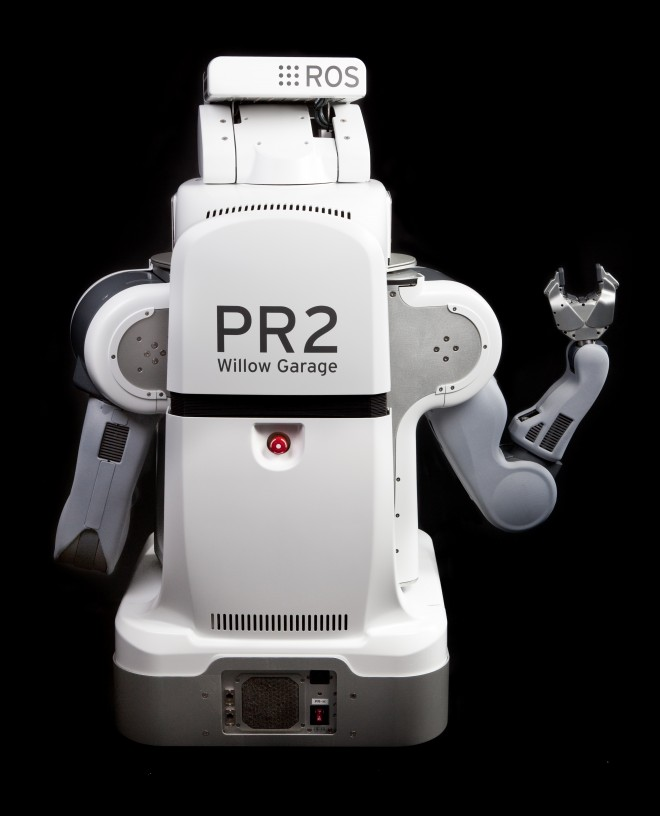
\includegraphics[height=45mm]{PR2-1}}
	\hspace{5mm}
	\subfigure[]{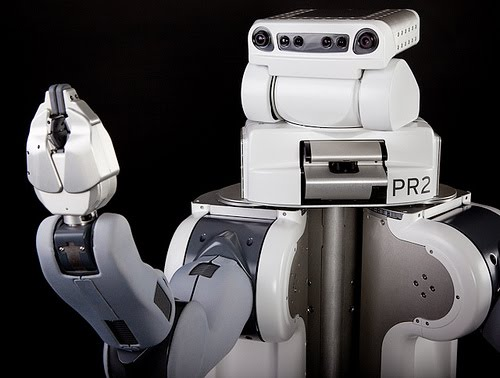
\includegraphics[height=45mm]{PR2-2}}
	\hspace{5mm}
	\subfigure[]{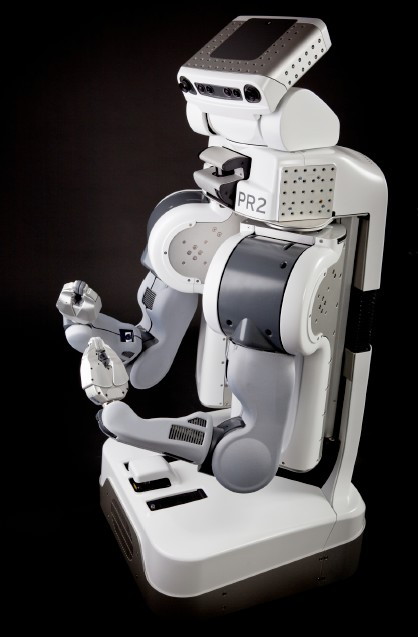
\includegraphics[height=45mm]{PR2-3}}
	\caption{PR2-Roboter (Quelle: Willow Garage)}
	\label{fig.PR2}
	\end{center}
	\vspace*{-8mm}
\end{figure}




Ausgestattet ist der PR2 mit zwei Armen, die jeweils sieben Freiheitsgrade haben und an deren Enden ein Greifer montiert ist, siehe \bild{PR2}. Die Sensorik des Armes besteht aus einer Kamera am Unterarm und Druck- sowie Beschleunigungssensoren am Greifer. Die Nutzlast eines Arms ist mit \SI{1,8}{\kilo\gram} ausgewiesen. Weiterhin verf�gt der Roboter �ber einen dreh- und schwenkbaren Kopf, in dem eine 5-Megapixel Farbkamera, ein LED-Texturprojektor und zwei Stereokameras integriert sind, wobei eine Kamera f�r die Fernsicht und die andere f�r die Objektmanipulation genutzt wird. Unterhalb des Kopfes ist ein schwenkbarer Laserscanner und ein Inertialsensor verbaut. Die Position des Oberk�rpers l�sst sich in der H�he zwischen \SI{1330}{\milli\meter} und \SI{1645}{\milli\meter} (Gesamth�he) variieren. Angetrieben wird die omnidirektionale Basis von vier gelenkten R�dern, die eine maximale Geschwindigkeit von \SI{3,6}{\kilo\meter\per\hour} erm�glichen. Die quadratische Basis hat eine Kantenl�nge von \SI{668}{\milli\meter}. Als Recheneinheit stehen zwei Server zur Verf�gung, die jeweils auf acht CPU-Kernen rechnen und dabei auf 24\,GB Arbeitsspeicher zugreifen k�nnen. Als Betriebssystem wird Ubuntu verwendet, auf dem das Robot Operating System, kurz ROS, die Grundlage f�r die Datenverarbeitung bildet. Da ROS innerhalb dieser Arbeit ebenfalls zum Einsatz kommt, wird dieses in \Sec{IntroductionROS} vorgestellt und an den entsprechenden Stellen weiter erl�utert. Die Kosten f�r einen PR2-Roboter belaufen sich derzeit auf etwa \SI{400.000}{US-Dollar}\footnotemark. Mit Hilfe des PR2 wurden von den zuvor erw�hnten Beta-Testern Szenarien bew�ltigt, die innerhalb des menschlichen Wohnraumes auftreten k�nnen. An der TU M�nchen hat ein PR2-Roboter beispielsweise zusammen mit einem anderen Robotersystem einen Pfannkuchen gebacken \cite{TUM2011}.
\footnotetext{Der angegebene Preis wurde am 16.08.2011 der Website http://www.willowgarage.com/pages/pr2/order entnommen und versteht sich exklusive Steuern und Versandkosten.}

\section{Technische Daten der youBot-Plattform}

\begin{table}[ht]
	\centering
	\caption{Technische Daten der youBot Plattform}\label{tab.TechSpecYouBotBase}
	\vspace*{-3mm}
	\begin{longtable}[ht]{|l|c|r|}\hline
		\rowcolor{Snow2}
		Bezeichnung						& Formelzeichen	& \\ \hline
		Gesamtl�nge 					&			& \SI{530}{\milli\meter}				\\ \hline
		Gesamtbreite 					&  		& \SI{350}{\milli\meter}				\\ \hline
		H�he									&  		& \SI{106}{\milli\meter}				\\ \hline
		Radstand							& $l$	& \SI{470}{\milli\meter}				\\
		\hline
	\end{longtable} 
	\vspace*{-3mm}
\end{table}


\begin{lstlisting}[label=source.launchHokuyo,caption=Launchfile zum Start der hokuyo\_node]
<!-- launch hokuyo node -->
<node pkg="hokuyo_node" type="hokuyo_node" name="hokuyo_node" output="screen">
	<param name="port" value="/dev/ttyACM0"/>
	<param name="frame_id" value="/base_laser_front_link"/>
</node>
\end{lstlisting}
    %\include{aufbau}
    %\include{versuchsdurchfuehrung}
    %\include{ergebnisse}
    %\include{schlusswort}
    %\nocite{*}                             % alle Literaturquellen einbinden, sonst werden nur die zitierten
                                            % Quellen im Literaturverzeichnis angezeigt (ist Geschmackssache).
                                            % eher nicht verwenden, au�er man hat einen guten Grund
    \appendix                               % Anhang starten, jedes weitere Kapitel bekommt jetzt einen Buchstaben
    \chapter*{Anhang}                       % Anhang als Chapter
    \thispagestyle{empty}                   % keine Kopfzeile, Seitenzahl u.a., leere Seite mit �berschrift Anhang
    \setcounter{chapter}{1}                 % Chapter Counter auf 1 = im Anhang A
    \setcounter{equation}{0}                % Equation Counter nullen
    \addstarredchapter{Anhang}              % Minitoc mitteilen, dass neues Chapter
    \newpage                                
    \ihead{\normalfont Anhang}              % Kopfzeile auf Anhang setzen
    
    \minitoc                                % Anhangsverzeichnis plotten
    %% --- Ab hier der Anhang einf�gen

    %\include{anhang_wheatstone}            % Anhang
    %\include{anhang_fehlerfortpflanzung}
		%\include{anhang_mgcEinstellungen}
		%\include{anhang_trafos}
		%\include{anhang_befestigen}
		%\include{anhang_datenblaetter}
  

    %% --- Anhang zu Ende
    \ihead{\normalfont\headmark}            % kolumnentitel innen
 
    %% --- Literaturverzeichnis
    \bibliographystyle{alphadin}            % Darstellung nach DIN, mit Name und Jahr z.B. [Sch06]
    \bibliography{masterbib}                % Literaturverzeichnis einbinden

\end{spacing}
\end{document}                              % fertig!

